\documentclass[11pt]{article}
\usepackage{../../timestamp}
\usepackage{../../astro207}
\usepackage{../../markup}
\usepackage{../../fa21}
\usepackage{tikz}
\usetikzlibrary{calc,shapes.geometric,arrows,automata}
\usepackage{color,hyperref,listings,enumitem}
\usepackage{algorithm}
\usepackage{algpseudocode}
\usepackage{tkz-euclide}
\usepackage{pgfplots}
\usepackage{pdfpages}
\usepackage{bm}
\usepackage[american,siunitx]{circuitikz}
\lstset{basicstyle=\ttfamily}
\newcommand{\fillin}[1]{\underline{\hskip #1}}
\newcommand{\doublehrule}{\hrule \vskip 0.02in \hrule}
\newcommand*\circled[1]{\tikz[baseline=(char.base)]{
  \node[shape=circle,draw,inner sep=2pt] (char) {#1};}}
\usepackage{hyperref}
\hypersetup{
	colorlinks=true,
	linkcolor=black,
	urlcolor=blue
}

\begin{document}

\def\title{Problem Set 2}
% \config{hwnum}{1}
% \config{homework-due}{08/31/2018 23:59}
% \config{grades-due}{09/04/2018 23:59}

\newcommand{\qitem}{\qpart\item}

\renewcommand{\labelenumi}{(\arabic{enumi})} % change default enum format to (1)
\renewcommand{\theenumi}{(\arabic{enumi})} % fix reference format accordingly.
\renewcommand{\labelenumii}{\roman{enumii}.} % second level labels.
\renewcommand{\theenumii}{\roman{enumii}.}

\maketitle
\begin{qunlist}

\qns{Blackbody Flux}

\ans{
	\begin{align*}
		B_\nu &= \frac{2h\nu^3}{c^2}\frac{1}{e^{\frac{h\nu}{k_BT}}-1}\\
		\int_{0}^\infty\int_{0}^{2\pi}\int_{0}^{\pi/2}B_\nu\cos\theta\sin\theta d\theta d\phi d\nu &= 2\pi\int_{0}^{\pi/2}\cos\theta\sin\theta d\theta \int_{0}^\infty B_\nu d\nu\\
			&= 2\pi \cdot \frac{1}{2} \cdot\int_0^\infty \frac{2h\nu^3}{c^2}\frac{1}{e^\frac{h\nu}{k_BT} - 1}d\nu\\
			&= \pi \int_0^\infty \frac{2h\frac{c^3}{\lambda^3}}{c^2}\frac{1}{e^\frac{hc}{\lambda k_BT}-1} d\nu \\
			&= \pi \int_0^\infty \frac{2hc^2}{\lambda^5}\frac{1}{e^\frac{hc}{\lambda k_BT}-1} d\lambda \longleftarrow \begin{cases}\nu = \frac{c}{\lambda}\\d\nu = -\frac{c}{\lambda^2}d\lambda\end{cases}\\
			&= \pi \cdot 2hc^2 \cdot \frac{hc}{k_BT} \cdot \left(\frac{k_BT}{hc}\right)^5 \int_0^\infty \frac{1}{x\left(e^{1/x}-1\right)}dx \longleftarrow \begin{cases}x = \lambda \frac{k_BT}{hc}\\dx = d\lambda\frac{k_BT}{hc}\end{cases}\\
			&= \pi \cdot \frac{2k_B^4T^4}{h^3c^2}\cdot \frac{\pi^4}{15}\\
			&= \frac{2\pi^5k_B^4}{15h^3c^2}T^4\\
			&= \sigma T^4
	\end{align*}
\textcolor{white}{And of course I forgot the Jacobian the first time around}
}
\newpage
\qns{Flat Disks}

\work{
	For an annulus in the ring at distance $r$, power in must equal power out
	\begin{align*}
		P_\text{in} &= P_\text{out}\\
		F_\text{in} &= F_\text{out}\\
			&= \sigma T^4
	\end{align*}
	where $T$ is the temperature in question.
	For the flux coming from the star where $\tan\theta_c = \frac{R_*}{r}$,
	\begin{align*}
		F_\text{in} &\approx F_*\cdot 4\pi R_*^2 \cdot \frac{1}{4\pi r^2} \cdot C\sin\theta_c\\
			&\approx \sigma T_*^4\frac{R_*^2}{r^2}\frac{R_*}{r}
	\end{align*}
	where $C$ (roughly 1) accounts for error from $r-R_* \approx r$ and the fact that there should be an integral over $\theta$ going from $0$ to $+\theta_c$.
	\begin{align*}
		\sigma T^4 &\approx \sigma T_*^4\frac{R_*^2}{r^2}\frac{R_*}{r}\\
		T &\approx T_*\left(\frac{R_*}{r}\right)^\frac{3}{4}
	\end{align*}
	\textcolor{red}{This feels weird, but I guess as you get further away a slice of the ring of the same area occupies a smaller solid angle from the view of some $z\neq 0$ point on the star?}}

\ans{
	$$T \approx T_*\left(\frac{R_*}{r}\right)^\frac{3}{4}$$
}

\sol{
	Starlight strikes the flat disk not at normal indicdence, but rather at grazing incidence.
	A quick but crude way to solve this problem proceeds as follows.
	Imagine that you are a path of unit area lying in the flat disk. 
	From your perspective, you see the upper half face of the star.
	Idealize the upper half face of the star as a single point source lying above the disk plane at height $\approx R_*$.
	We should model this point source as having a luminosity of order $\frac{1}{2}$ the luminosity of the total star, because we can only see the upper half face of the star (if the bottom of the disk were onot there, we could see the entire half face of the star).

	Naively (and incorrectly), we would say that the flux of light from this source, evaluated a distance $r$, would be $\frac{L_*/2}{4\pi r^2}$, where $L_*$ is the total luminosity of the star.
	But this would be incorrect, because what we really want is the flux of light passing through the flat patch of the disk.
	This is the light that the disk actually absorbs.
	The amount of energy crossing the flat patch per time equals $\frac{L_*/2}{4\pi r^2}$ TIMES the sine of the angle at which rays from the point source strike the patch.
	This angle is not 90\si{\degree} (normal indicidence), but rather is equal to $\approx \frac{R_*}{r}\ll 1$ (Fig. \ref{fig:flat_disks}).

	\begin{figure}[h]
		\centering
		\caption{\textcolor{red}{TODO}}
		\label{fig:flat_disks}
	\end{figure}

	Therefore, the true flux passing through the patch equals
	\begin{align*}
		\frac{L_*/2}{4\pi r^2}\cdot \frac{R_*}{r} &= \sigma T^4 \longleftarrow \text{flux absorbed equal to flux emitted by the patch}\\
		T &= \left(\frac{1}{2}\right)^\frac{1}{4}T_*\left(\frac{R_*}{r}\right)^\frac{3}{4}\longleftarrow L_* = 4\pi R_*^2\sigma T_*^4
	\end{align*}
	Note that the index for the radial scaling is 3/4, not 1/2.
	The temperature decays more steeply with distance for a flat disk than for, say, a system of planets because rays strike the disk at grazing incidence, not at normal incidence.

	We can redo this problem more carefully by integrating over the upper half face of the star rather than by idealizing the upper half face as a single point source.
	The result of such an integration is to replace the $(1/2)^\frac{1}{4}$ numerical coefficient above with $\left(\frac{2}{3\pi}\right)^\frac{1}{4}$.
}
\newpage
\qns{A Simplified Greenhouse Effect}

\work{
	\textcolor{red}{I suppose we'll assume the atmosphere doesn't emit as a blackbody and Earth doesn't reflect anything coming off of the sun?}
	\begin{center}
		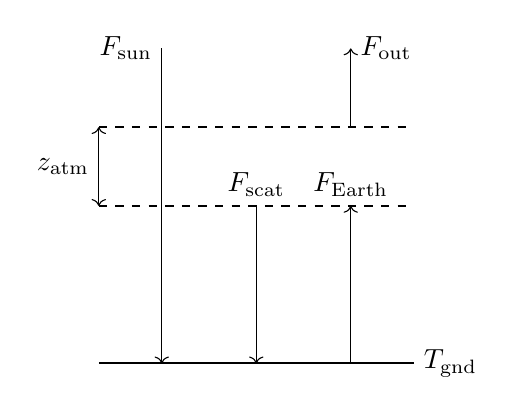
\begin{tikzpicture}
		% atmosphere
		\draw[dashed,line width=0.25mm] (-1,3) coordinate (atTopLeft) 
			-- ++(4,0) coordinate (atTopRight);
		\draw[dashed,line width=0.25mm] (atTopLeft)++(0,-1) coordinate (atBotLeft) 
			-- (atBotLeft-|atTopRight) coordinate (atBotRight);
		\draw[<->] (atTopLeft) -- (atBotLeft);
		\draw ($(atTopLeft)!0.5!(atBotLeft)$) node[anchor=east] () {$z_\text{atm}$};
		
		% ground
		\draw[line width=0.25mm] (atBotLeft)++(0,-2) coordinate (gndLeft) 
			-- (gndLeft-|atTopRight) coordinate (gndRight) node[anchor=west] () {$T_\text{gnd}$};
		
		% from sun
		\draw[->] ($(atTopLeft)!0.2!(atTopRight)$)++(0,1) coordinate (sunStart) 
			-- (sunStart|-gndLeft) coordinate (sunStop);
		\draw (sunStart) node[anchor=east] () {$F_\text{sun}$}; 

		% earth blackbody
		\draw[->] ($(gndRight)!0.2!(gndLeft)$) coordinate (earthStart)
			-- (earthStart|-atBotRight) coordinate (earthStop);
		\draw (earthStop) node[anchor=south] () {$F_\text{Earth}$};

		% scattering
		\draw[->] ($(atBotLeft)!0.5!(atBotRight)$) coordinate (scatStart)
			-- (scatStart|-gndLeft) coordinate (scatStop);
		\draw (scatStart) node[anchor=south] () {$F_\text{scat}$};

		% top of atmosphere
		\draw[->] (atTopRight-|earthStart) coordinate (outStart)
			-- (outStart|-sunStart) coordinate (outStop);
		\draw (outStop) node[anchor=west] () {$F_\text{out}$};
\end{tikzpicture}
	\end{center}
	\begin{align*}
		F_\text{Earth} = \sigma T_\text{gnd}^4 &= F_\text{scat} + F_\text{sun}\\
		\alpha &= n\sigma_\text{scat} = \frac{N}{z_\text{atm}}\sigma_\text{scat}
	\end{align*}
	We consider the amount of energy scattered back by a volume of scatterers depth $z$.
	\begin{multicols}{2}
		\raggedcolumns
		\begin{center}optically thin\end{center}
		$$z = z_\text{atm}$$
		Here we treat some constant fraction of energy which doesn't reach depth $s \in (0,z_\text{atm}]$ can be as scattered and assume extinction along the back-path isn't significant given the short distance.
		\vfill\columnbreak
		\begin{center}optically thick\end{center}
		$$z = \lambda_\text{mfp} = \frac{1}{n\sigma_\text{scat}} = \frac{z_\text{atm}}{N\sigma_\text{scat}}$$
		This isn't an unreasonable assumption, given backscattering within the atmosphere necessarily deals with extinction with the decaying exponential on the path back out of the atmosphere. 
	\end{multicols}
	\begin{multicols}{2}
		\raggedcolumns
		\begin{align*}
			F_\text{scat} &= F_\text{Earth}\left(1-k_\text{thin}e^{-\alpha z_\text{atm}}\right), 0 < k_\text{thin} < 1\\
			F_\text{Earth} &= F_\text{Earth}\left(1-k_\text{thin}e^{-\alpha z_\text{atm}}\right) + F_\text{sun}\\
			\sigma T_\text{gnd}^4 &\propto e^{N\sigma_\text{scat}}
		\end{align*}
		\vfill\columnbreak
		\begin{align*}
			F_\text{scat} &= F_\text{Earth}(1-k_\text{thick}), 0 < k_\text{thick} < 1/e\\
			F_\text{Earth}(k_\text{thick}) &= F_\text{sun}\\
			T_\text{gnd}^4 &\propto \text{constant}
		\end{align*}
	\end{multicols}
	% Considering $j_{\nu,\text{scat}} = n\sigma_\text{scat}J_\nu = \frac{N}{z_\text{atm}}\sigma_\text{scat}J_\nu$,
	% $$j_{\nu,\text{scat}}V_\text{scat} \propto \begin{cases}NJ_\nu & \text{optically thin}\\ J_\nu & \text{optically thick}\end{cases}$$
	% where $J_\nu = KF_\text{Earth}$ for some scalar $K$.
	% \begin{align*}
	% 	F_\text{Earth} &= F_\text{scat} + F_\text{sun}\\
	% 	\sigma T_\text{gnd}^4 &= F_\text{scat} + F_\text{sun}\\
	% 	\sigma T_\text{gnd}^4 &= \begin{cases}
	% 		\sigma T_\text{gnd}^4C_\text{thin}N + F_\text{sun} & \text{optically thin}\\
	% 		\sigma T_\text{gnd}^4C_\text{thick} + F_\text{sun} & \text{optically thick}\end{cases}
	% \end{align*}
	% where $C_\text{thick/thin}$ are constants.
}

\ans{
	\centering
	\begin{align*}
		T_\text{gnd} &\propto \begin{cases}
			\sqrt[4]{e^{N\sigma_\text{scat}}} & \text{optically thin}\\
			\text{constant} & \text{optically thick}
			\end{cases}
	\end{align*}}

\sol{
	If the entire atmosphere is in bolometric (i.e. frequency-integrated or total-energy) equilibrium, then at every point in the atmosphere, the going-down flux of incoming energy must be balanced by the up-going flux of outgoing energy.
	By the planar symmetry of the problem, we know that there cannot be any dependence on angle or position (other than vertical distance above the plane).
	Antoehr way of saying this: For every component of flux that is not normal to the plane above some position, a nearby position will have a symmetrical flux that cancels it out.

	At the outermost layer of the atmosphere where there is no backscatter, we must have the incident flux from the sun, $F_\odot$, exactly balanced by the blackbody flux $\sigma_{SB}T^4$.
	If we are measuring the optical depth for an infrared photon to escape as $\tau = N\sigma$, then the $\tau = 0$ solution is
	\begin{align*}
		T &= \left(\frac{F_\odot}{\sigma_{SB}}\right)^\frac{1}{4}
	\end{align*}
	In the optically thin regime where $1 \gg \tau > 0$, we star to have some backscatter as infrared photons try to escape, and this backscattered light adds to the incident solar flux.
	Because we are so optically thin, $e^{-\tau} \approx 1-\tau$, so the flux leaving the outermost layer of the amosphere is attenuated by $1-\tau$ relative to the blackbody flux underneath.
	This means that $F_\odot = \sigma_{Sb}T^4(1-\tau)$, so
	\begin{align*}
		T &= \left(\frac{F_\odot}{\sigma_{SB}(1-N\sigma)}\right)^\frac{1}{4}
	\end{align*}
	This obviously perturbs the temperature slightly, but if forced to answer how $T$ scales with $N$, the fact that $N\sigma\ll 1$ means that it is effectively flat (the $N^0$ term dominates the Taylor expansion).

	In the optically thick regime, the exiting blackbody flux is attenuated by $e^{-\tau}$ and it really is in the exponential region this time: $\sigma_{SB}T^4 e^{-\tau} = F_\odot$, so
	\begin{align*}
		T &= \left(\frac{F_\odot e^{N\sigma}}{\sigma_{SB}}\right)^\frac{1}{4}
	\end{align*}
	This means that $T\propto e^\frac{N\sigma}{4}$.

	The point, in this simplified model, is that temperature goes from flat to exponential very rapidly with increasing column density as we cross the optically thin/thick boundary.
}
\end{qunlist}

\end{document}
